\chapter{Valutazioni}

Attraverso l'implentazione delle nuove funzionalità, il miglioramento dell'usabilità grazie allo sviluppo della nuova
interfaccia è stato possibile avere uno strumento di debug per leggere i messagi in Can-Bus,
salvarli grazie agli applicativi di \emph{canutils} e ottenere quindi uno software stabile per testare e fare operazioni di
debug sulla macchina.
Il Volante di Chimera Evoluzione è pienamente utilizzato in tutte le sue funzionalità ed è ritenuto lo strumento 
sviluppato dal team più stabile in macchina al momento. Questo oltre alle scelte tecniche prese che lo rendono performante 
in diverse situazioni, mostra i vantaggi nella sua architettura, cioè essere principalmente in lettura.

\begin{figure}[hbt!]
    \centering
    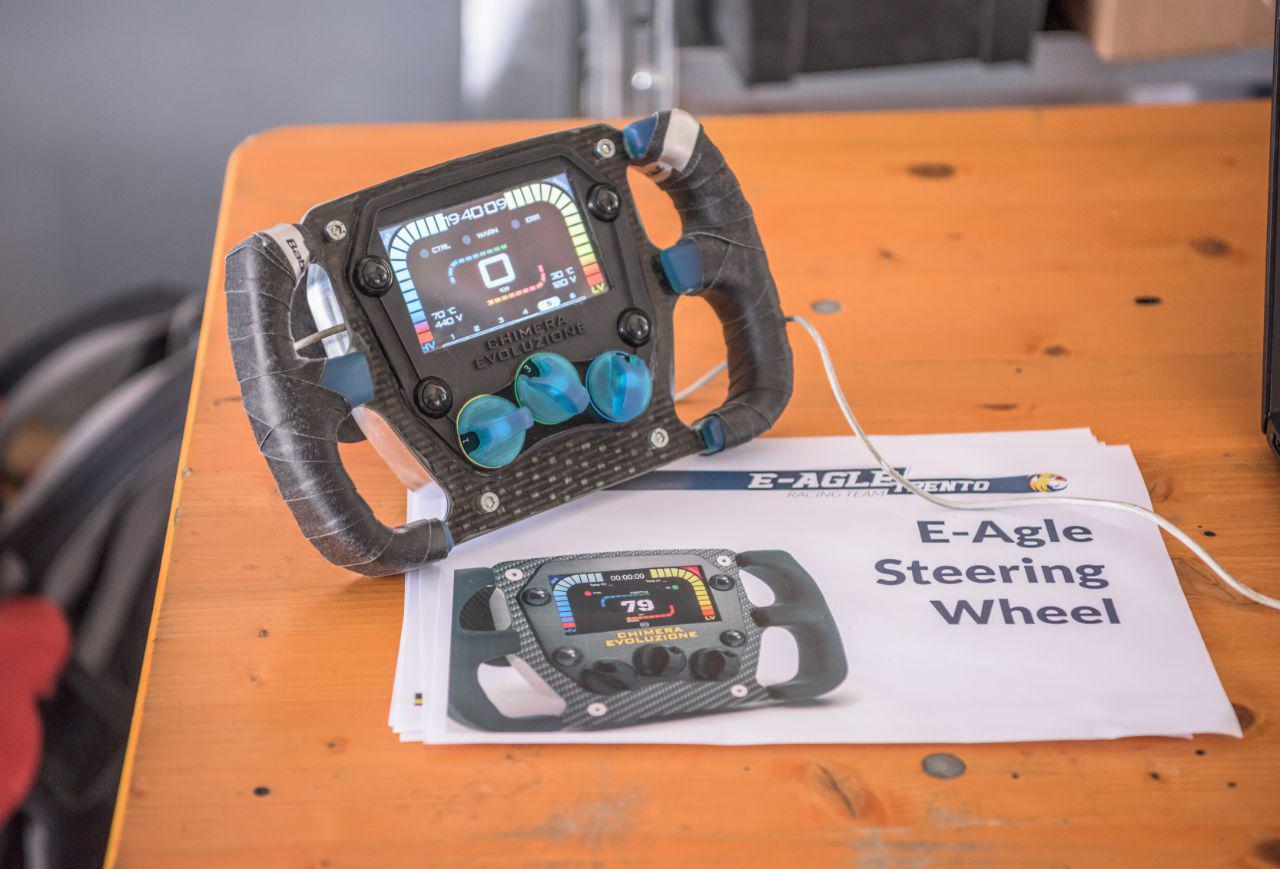
\includegraphics[width=0.75\textwidth]{./figures/steeringwheelPresentation.jpg}
    \caption{Presentazione del Volante - Varano Luglio 2018}
\end{figure}

Nel Luglio 2018, durante la partecipazione alla tappa italiana del campionato presso il circuito di Varano (PR), ho avuto la prima conferma da parte 
di esterni sulla qualità del nostro lavoro, delle scelte tecniche e di sviluppo che sono state fatte durante l'anno.
La riconferma di ciò è stata la premiazione da parte di Alessandro Pocecco, Project Leader della parte Elettronica di Lamborghini, 
con il premio per \emph{Best HMI Solution}.
La soluzione che abbiamo deciso di presentare è stata valutata non solo come prodotto, ma soprattutto per la presentazione che ho avuto
l'onore di condurre, mostrando in particolare il nostro approccio durante la fase di design del prodotto e le metodologia di sviluppo.
Il giudice si è complimentato per l'impegno, dandoci numerosi consigli e facendo apprezzamenti sulle scelte tecniche in base ai nostri requisiti,
che sono state motivate utilizzando un approccio molto più vicino al mondo lavorativo che a quello didattico.

Ad Agosto 2018, durante la tappa di Barcellona, ci è stato fatto presente della mancanza di una vera soluzione telemetrica, questo perchè il Volante
è stato pensato per essere utilizzato principalemente dal Pilota e per i test, ma non per la raccolta dati. 
Da qui è nata la necessità di sviluppare una appliciazione a microservizi basata sulla comunicazione wireless della macchina 
con un dispositvo esterno per raccoglierne i dati e visualizzarli in real-time con il salvataggio in database per poter poi fare delle analisi più
precise sulla nostra monoposto.

\section{Sviluppi Futuri}

Per quanto riguarda il Volante, grazie ai feedback dei giudici, delle persone che ci hanno lavorato come utenti e da chi l'ha sviluppato abbiamo raccolto
molte informazioni sul come poterlo migliorare.
Per poter avere un'analisi più precisa sulle risosrse da impiegare al miglioramente del dispositivo
abbiamo deciso di utilizzare un'approccio qualitativo diverso.
L'approccio consiste nel definire parametri misurabili in fase di progettazione, molto simile a quello utilizzato dal gruppo telemetria 
ma senza l'utilizzo di variabili.
Questa tecnica viene chiamata \textbf{QFD} e consiste nel tenere conto delle necessità del cliente esterno 
per poter venire il più possibile incontro a quelle del cliente interno (sviluppatori e designer).
È importante precisare che il nostro principale competitor siamo noi stessi, con la soluzione che abbiamo 
implementato nel 2018.
Al momento non sono presenti all'interno della competizione di Formula SAE prodotti custom simili al nostro,
curati sia dal punto di vista grafico che funzionale, ma soluzioni per il motor-sport in generale acquistate e utilizzate dalle squadre.

\begin{figure}[hbt!]
    \centering
    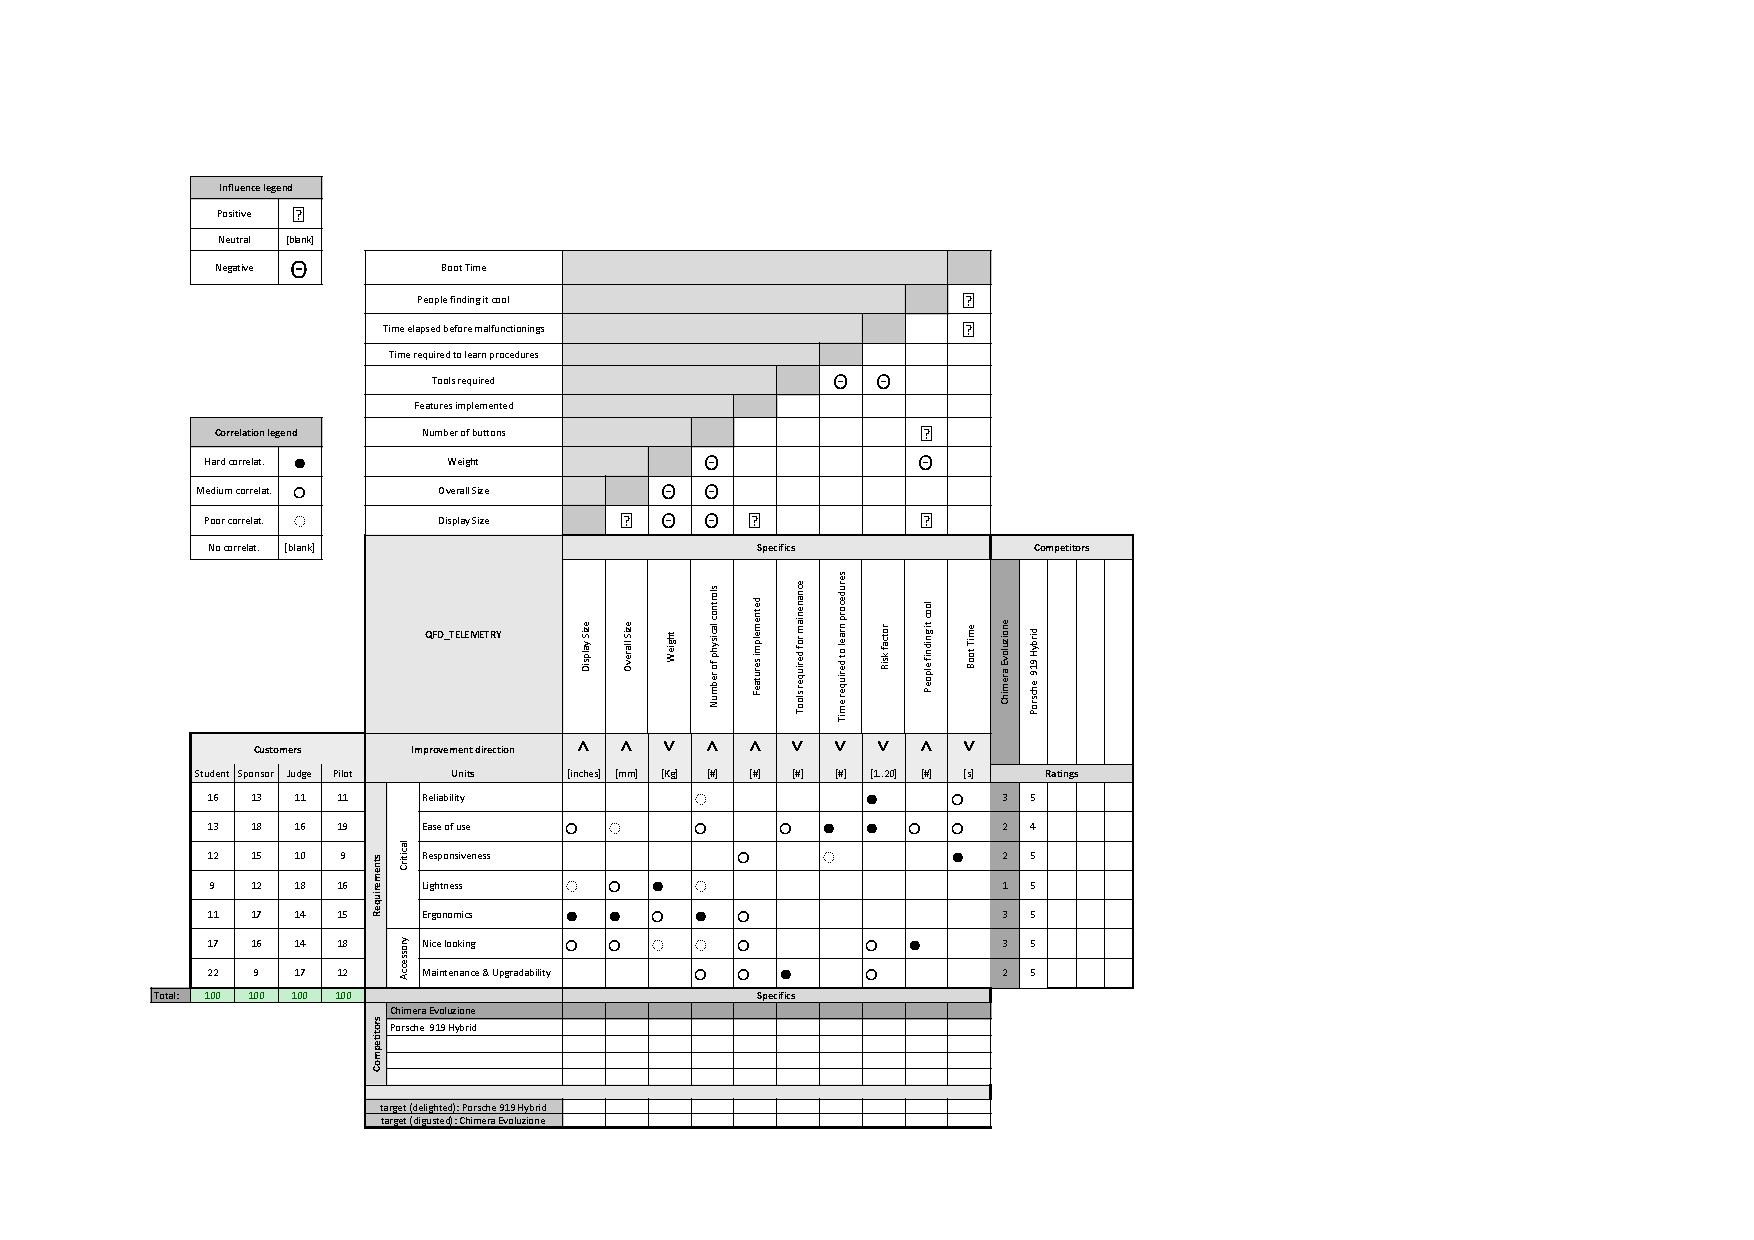
\includegraphics[width=0.95\textwidth]{./figures/QFD_Telemetry.pdf}
    \caption{QFD Ottobre 2018}
\end{figure}

Dalla QFD sono emersi diversi punti importanti su cui lavorare, qui schematizzati:

\begin{itemize}
    \item Case ridisegnato per renderlo facilemente aggiornabile grazie al ausilio di una 
            mascherina che può essere rimossa per poter lasciare il case uguale e ridurre i costi.
    \item Impugnatura ergonomica su misura ottenuta attraverso scanner 3D. 
    \item Cambiare hardware, scelta di una scheda più potente e ridurre lo spazio della componentistica hardware, 
        la soluzione di riferimento è un Raspberry Pi CM3 con memoria SD.
    \item Gestire su due Thread il programma, uno per la lettura del Can-Bus l'altro per l'interfaccia.
    \item Migliorare i tempi di boot del sistema operativo. Grazie al premio vinto 
        abbiamo potuto conttattare \emph{Qt} per una sponsorizzazione e ora abbiamo a disposizione 
        l'intera suite per lo sviluppo emebedded che, attraverso anche alla collaborazione dei loro
        partner, ci permetterà di utilizzare al massimo le potenzialità del loro framework.
    \item Aggiornare l'interfaccia proponendo più versioni in base al caso d'uso e il pilota.
    \item Inserire led di notifica sopra al display, questa funzionalità è ancora da definire ma una 
        sua prima applicazione può essere notificare certe informazioni al pilota o a 
        chi fa i test e in fase di gara vedere il bloccaggio delle ruote. 
    \item Aggiornare i dispositivi di input, inserendo altri due paddlee un bottone, uno per il launch control e 
        l'altro da utilizzare come marker (ripristinando la soluzione della comunicazione radio).
    \item Aumentare la dimensione del display da 4.3" a 5", per poter integrare nuove funzionalità e avere un display qualitativamente migliore.
    \item Rendere ancora più intuitiva l'interfaccia grazie a tasti con scritte colorate e automatizzare 
        alcune procedure alle quali il pilota non interessa conoscere attraverso un bottone di "start automatico", mantenendo e migliorando la veccia procedura.
    \item Aggiungere la possibilità di premere più tasti contemporaneamente per attivare altre funzioni.
    \item Migliroare il feedback per il pilota, attraverso il flash di colori e informazioni, 
        così da poter essere informati più velocemente sullo stato della macchina. 
\end{itemize}

\begin{figure}[h!]
    \centering
    \begin{minipage}{0.5\textwidth}
        \centering
        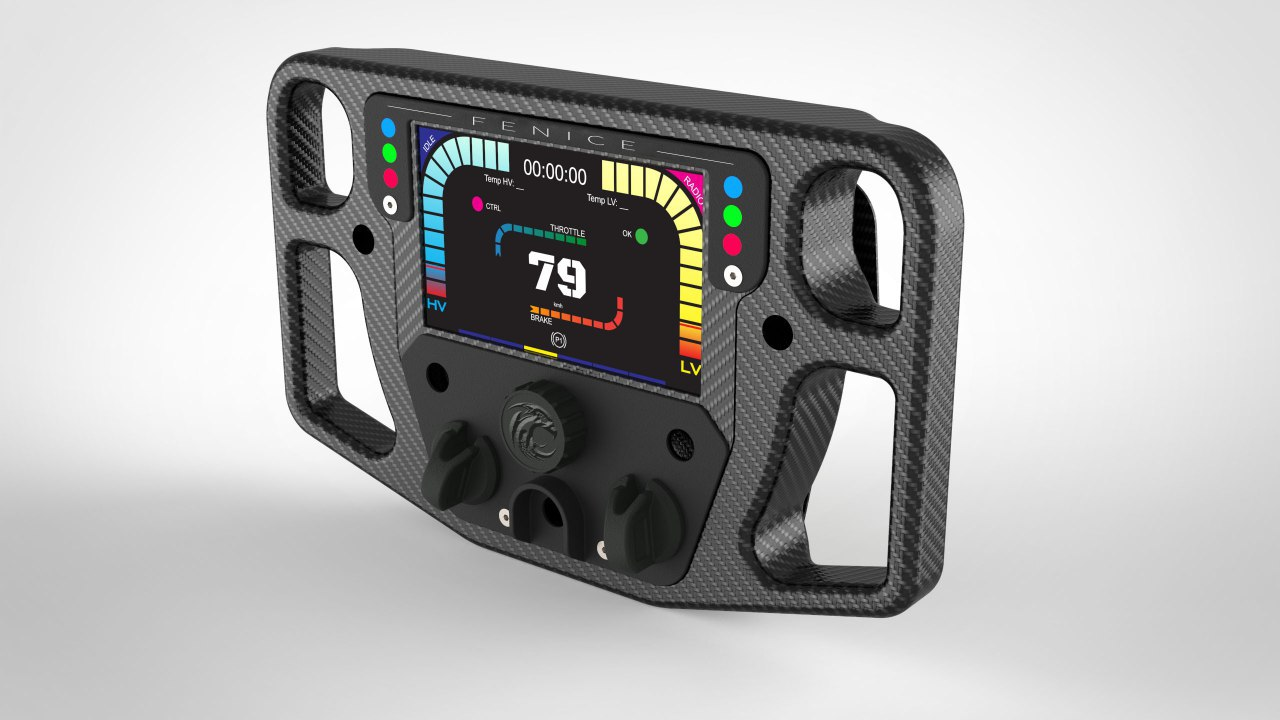
\includegraphics[width=0.9\textwidth]{./figures/volanteFenice.jpg}
    \end{minipage}\hfill
    \begin{minipage}{0.5\textwidth}
        \centering
        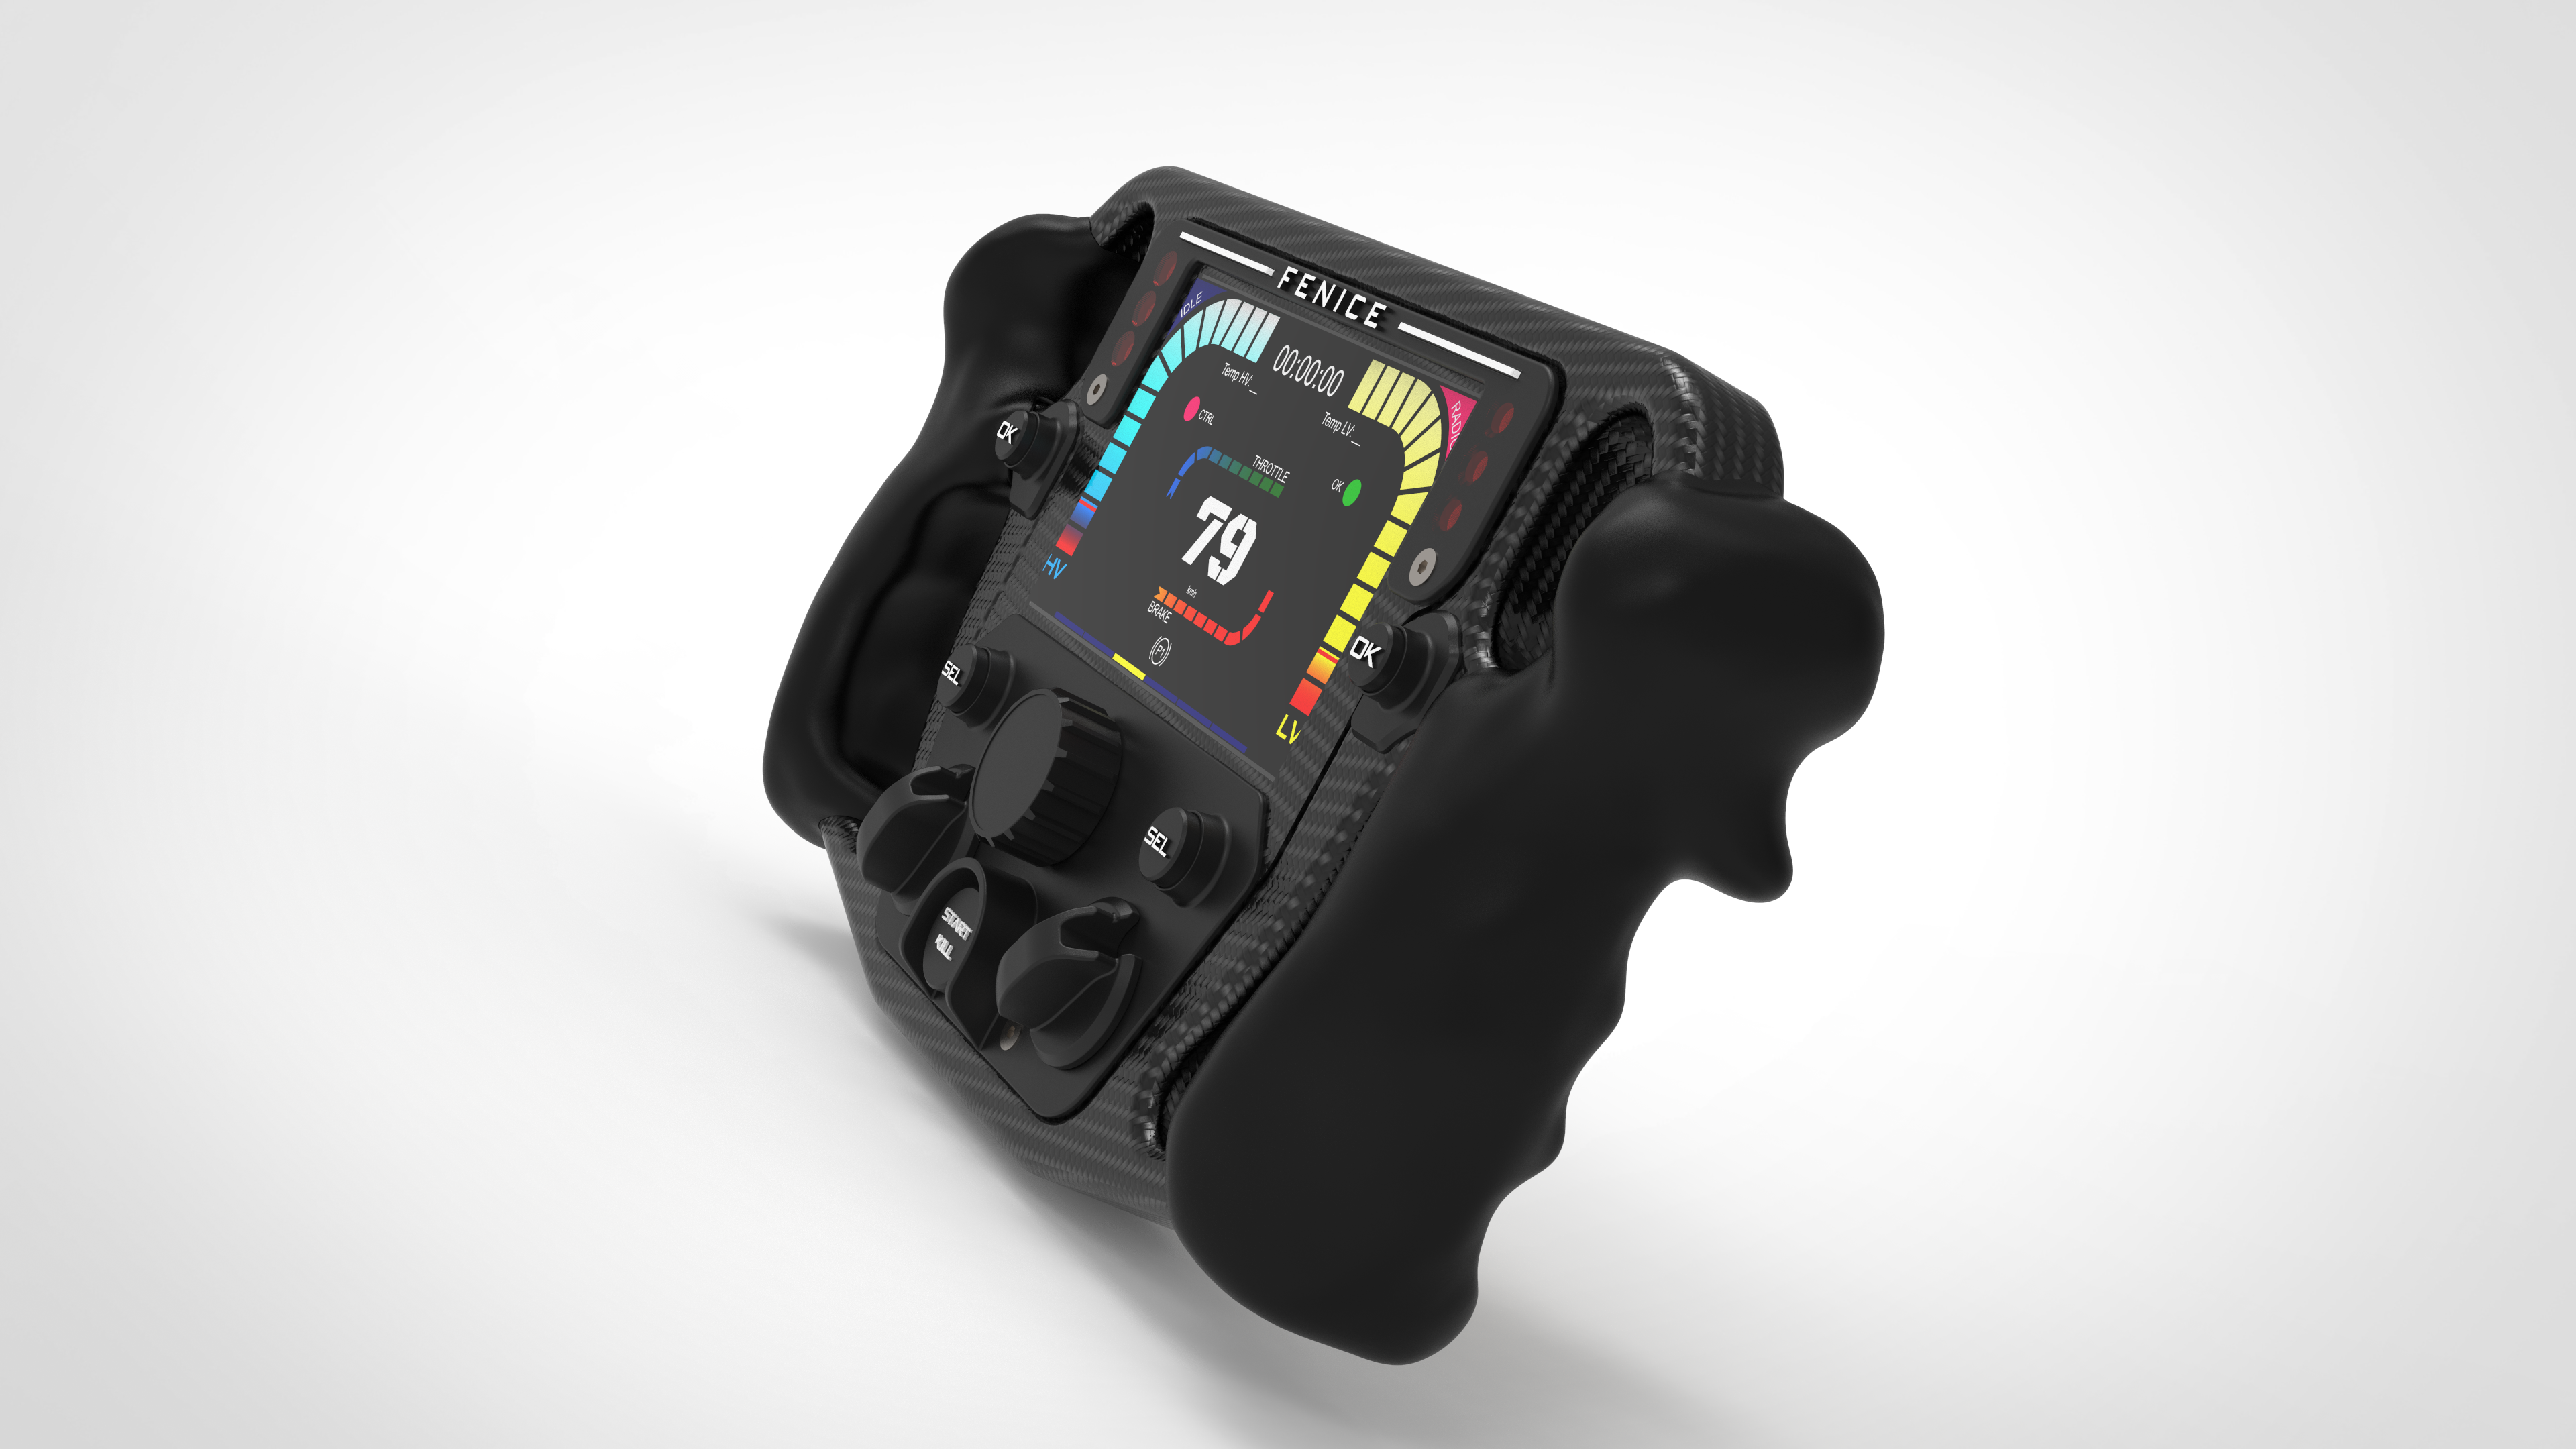
\includegraphics[width=0.9\textwidth]{./figures/volanteFenice1.png}
    \end{minipage}
    \caption{Primo Mockup del Volante di Fenice}
\end{figure}

% \begin{figure}[hbt!]
%     \centering
%     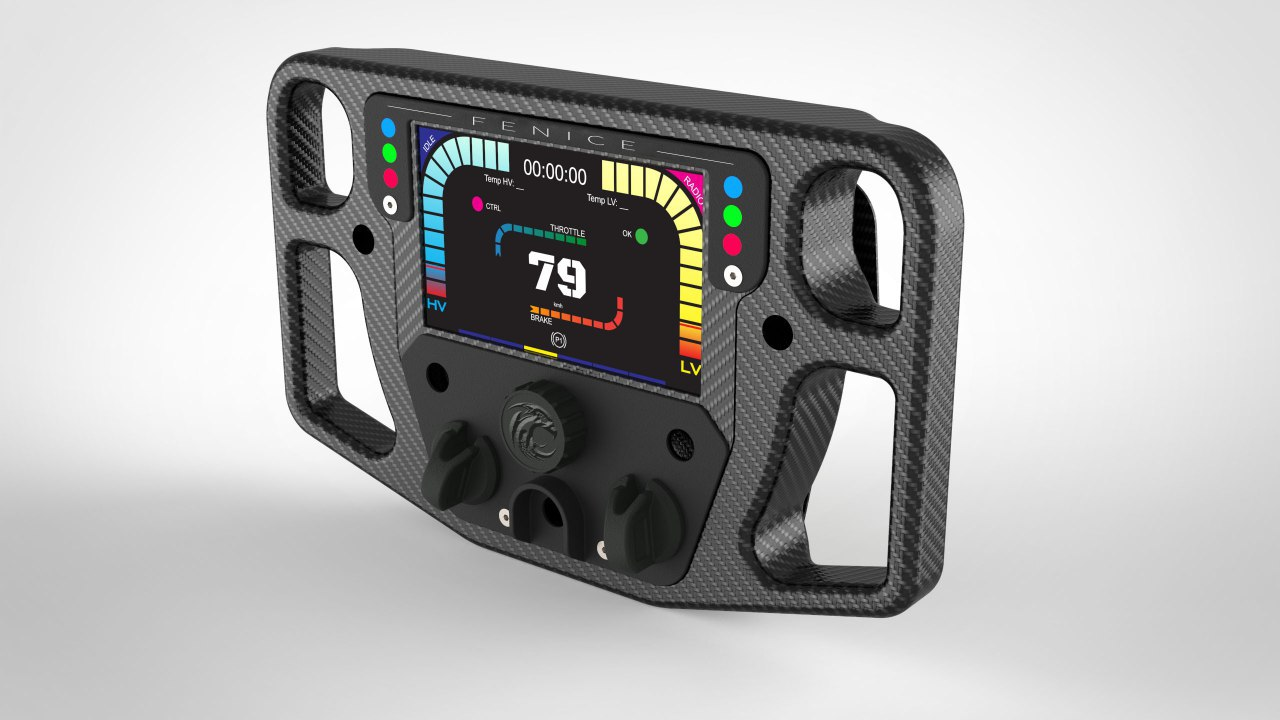
\includegraphics[width=0.75\textwidth]{./figures/volanteFenice.jpg}
%     \caption{Primo Mockup del Volante Fenice}
% \end{figure}

% \begin{figure}[hbt!]
%     \centering
%     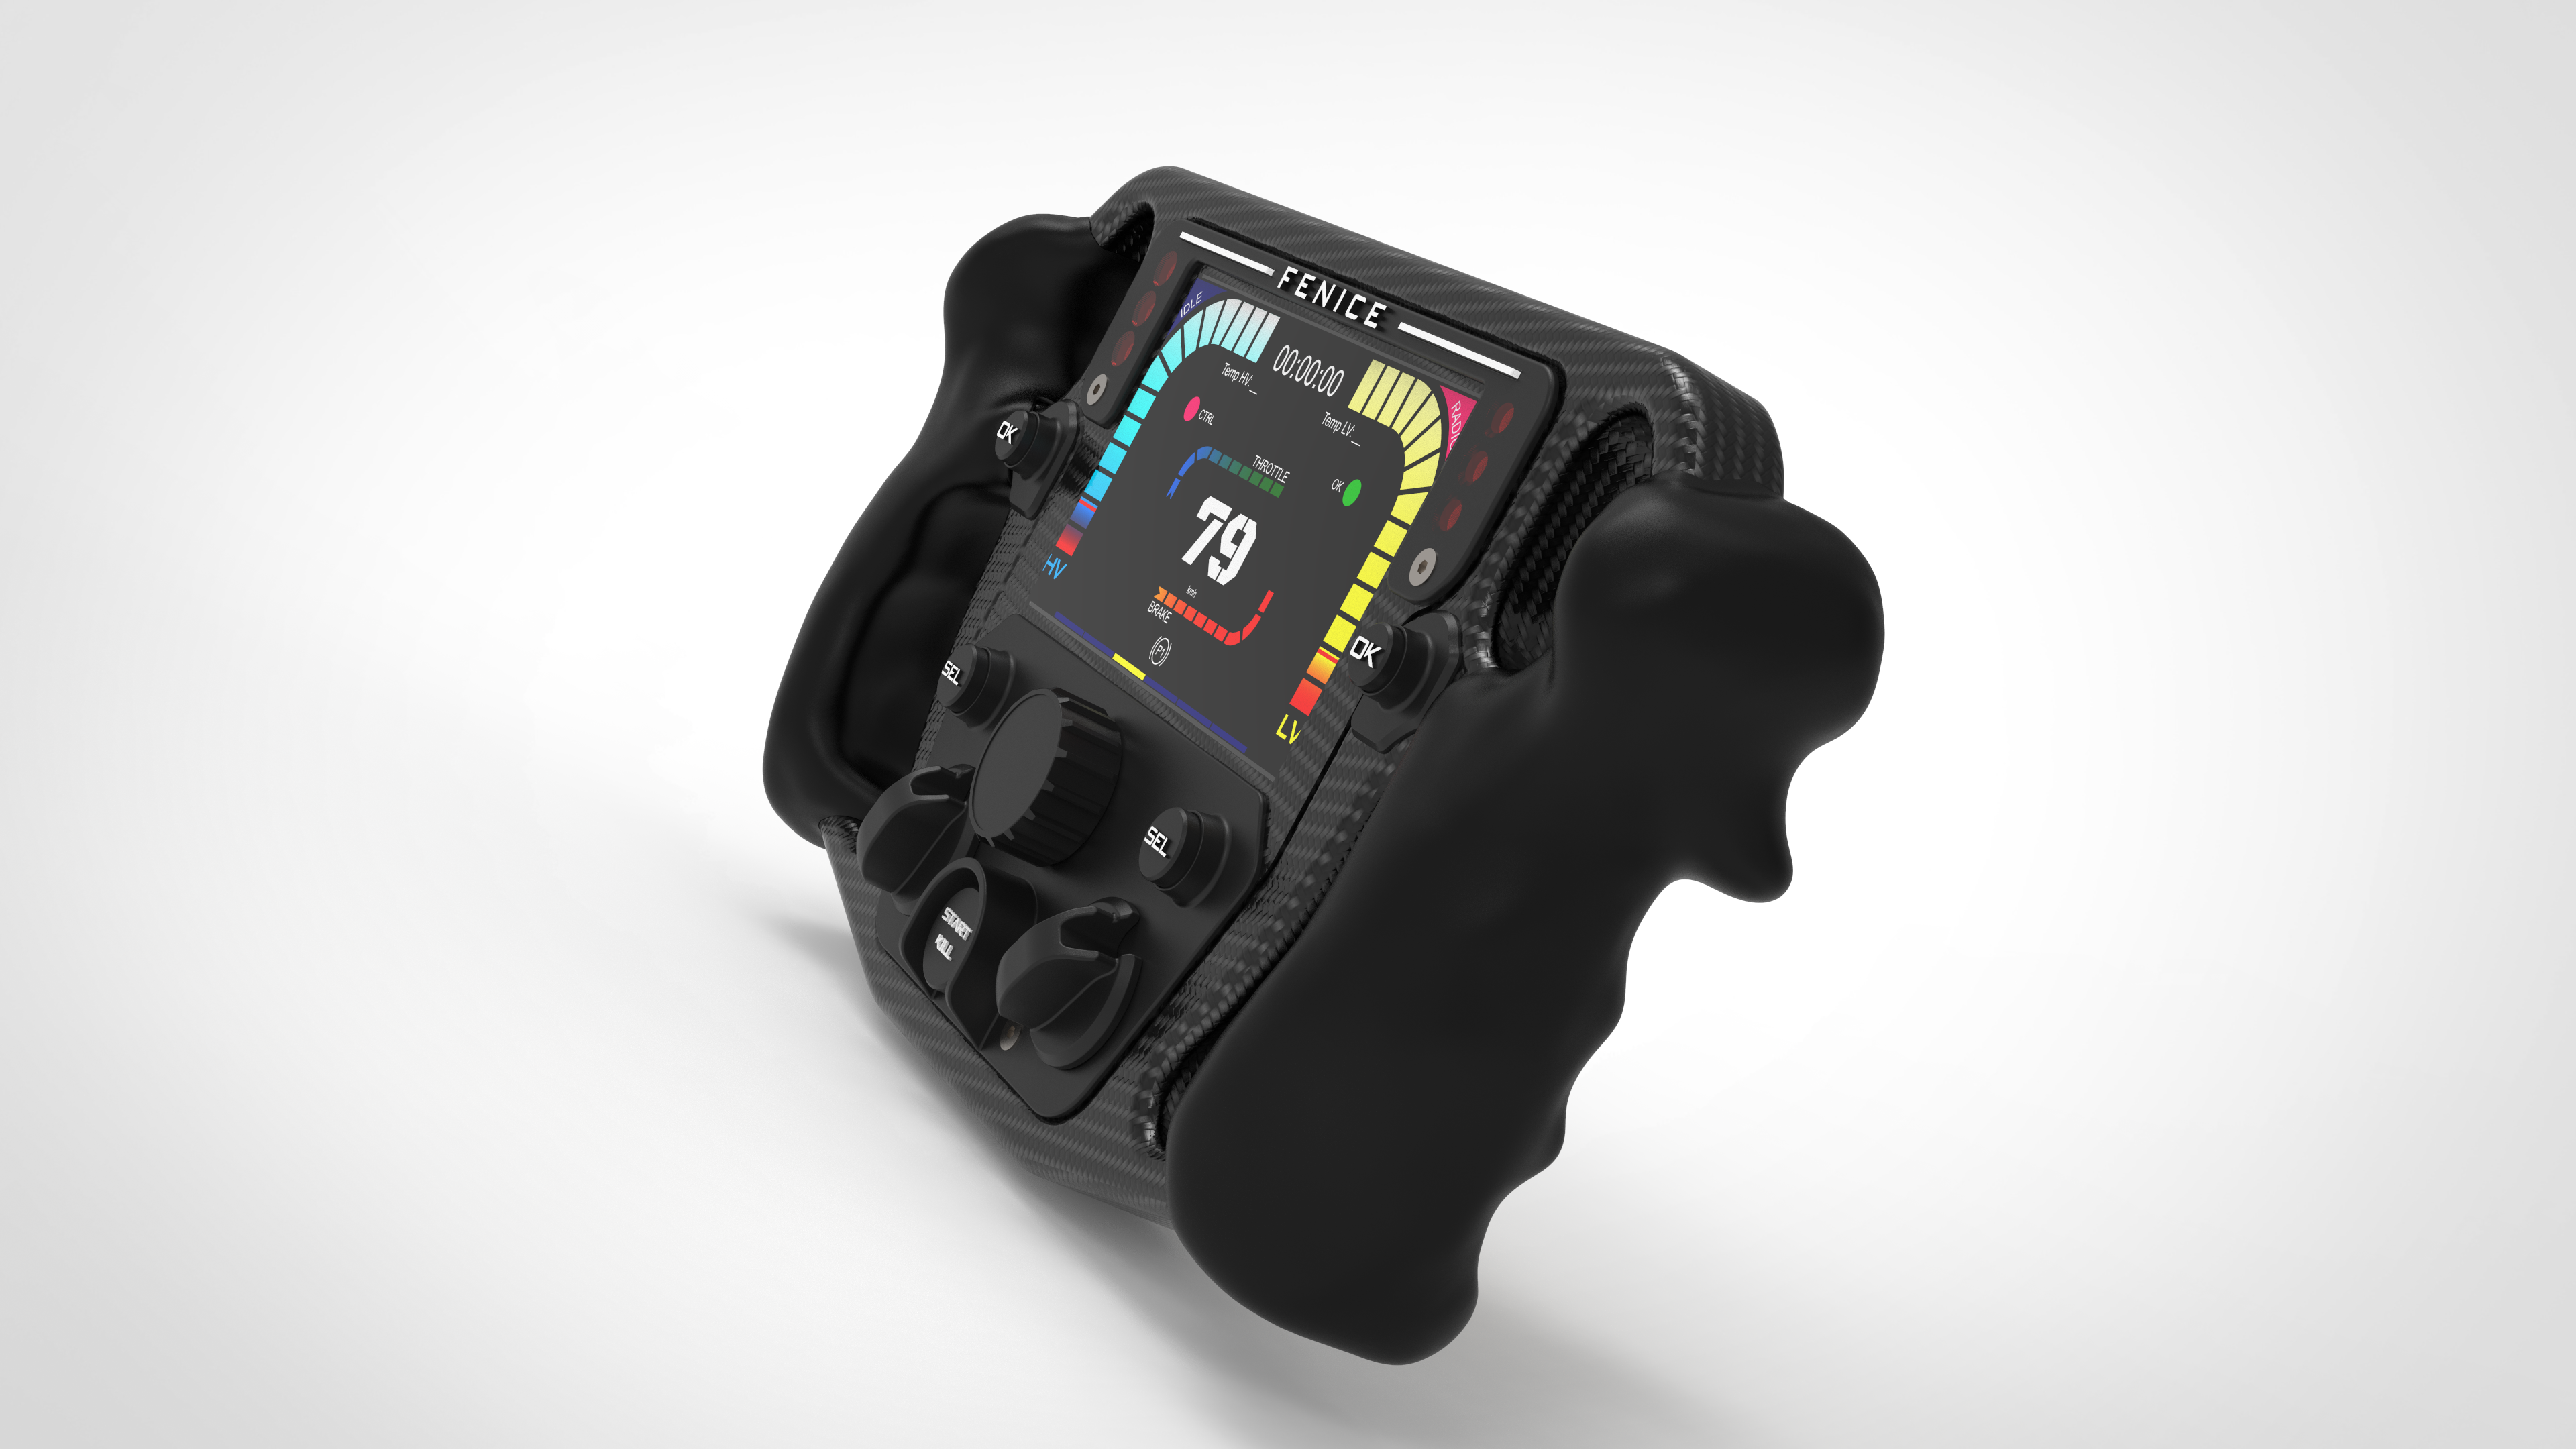
\includegraphics[width=0.75\textwidth]{./figures/volanteFenice1.png}
%     \caption{Impugnatura Ergonomica Scannerizzata 3D}
% \end{figure}

Il progetto del Volante non è da intedersi come finito, ma come continua ricerca di soluzioni migliori.
Il test su altri dispositvi e con altre tecnologie mostra la facilità/difficoltà di integrarsi al nostro progetto, 
la scelta di effettuare questo tipo di prove viene preso dal singolo valutando la fattibilità e l'interesse personale.
Un esempio è il framework che utilizza il gruppo Volkswagen, in particolare Audi con il loro premiato MMI. È sicuramente un ottima soluzione, ma le considerazioni fatte sui prezzi delle licenze,
il taget dei loro clienti (principalmente designer) ci ha spinto scartarlo optando per soluzioni open-source, poco costose e che sfruttano tecnologie che possono mostrarsi polifunzionali. 

\newpage

% \textbf{TODO del futuro}

% Attraverso queste funzionalità e design siamo riusciti ad avere: 
% \begin{itemize}
%     \item Toold Debug (canutils, candump, le tab)
%     \item Tool + stabile al momento in macchina (non si rompe in quanto è in lettura e mostra lo stato della macchina sempre)
% \end{itemize}

% mettere feedback del display per procedure
% ripensare alle procedure migliorando l'efficenza e limitare l'aggiornamento della grafica i 30fps 
% mettere su due thread la ui il backend

% problemi e come li risolviamo (fenice hw, so miglioratoe, nuove interfaccia 5", tasti colorati, notifica pressione tasti nuove funzionalità della telemetria) 
% approcio nuovo grazie alla sponsorizzazione di qt, valutazione anche di framework alternativi, vedi kanzi usata dal gruppo audi, ma più orientato ad un approccio 
% da desginer che da studenti di ingegeria, oltre a questo risulta essere costoso e "innarivabile" per il nostro progetto (volante) che si fonda sullo spendere
% il meno possibile e realizzare le migliori soluzioni dando il più possibile del nostro
